% !TeX spellcheck = en_GB
\chapter{Results}
\section{\SI{48}{\hour} surface observations and MEPS forecasts}%\hfill} 
\label{app:sfc_obs}
%%%%%%% image sfc obs  %%%%%%%%%%%%%%%%
\begin{figure}[H]
	\centering
	% sfc pressure
	\begin{subfigure}[b]{0.49\textwidth}
		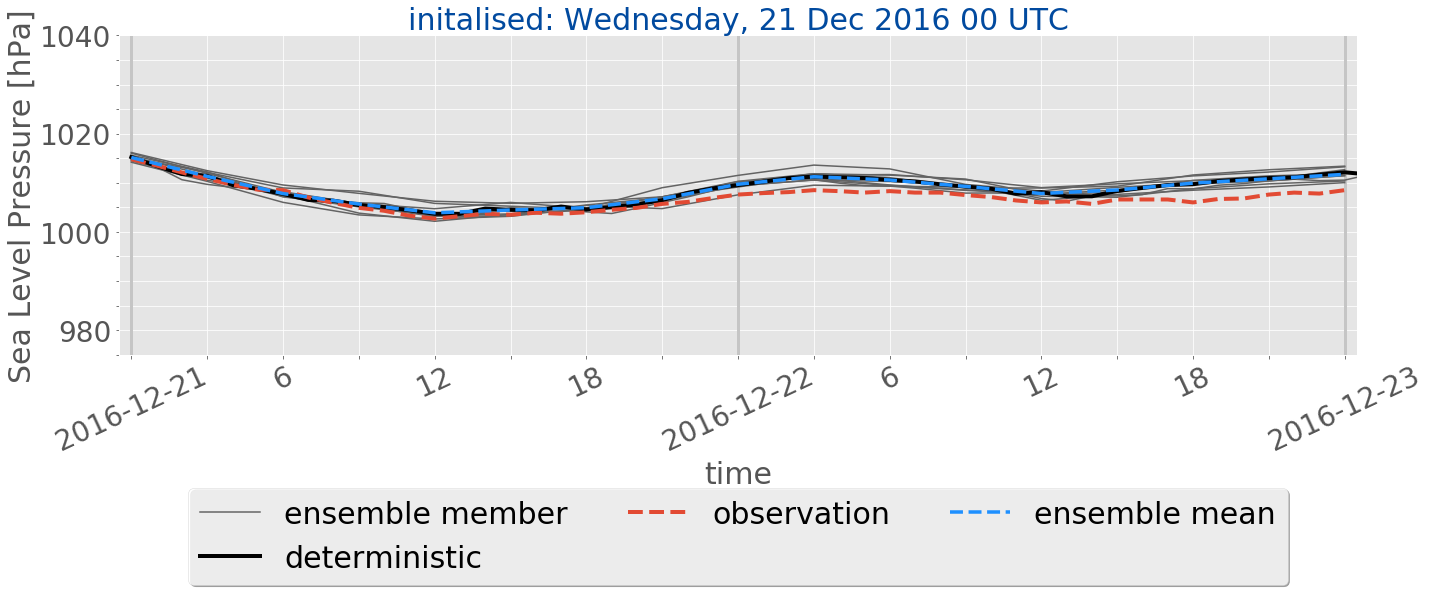
\includegraphics[trim={0.cm 5.cm 0cm 0cm},clip,
		width=\textwidth]{./fig_sfc_pressure/20161221_00}
		\caption{}\label{fig:res:sfc_pres21}
	\end{subfigure}
	%
	\begin{subfigure}[b]{0.49\textwidth}
		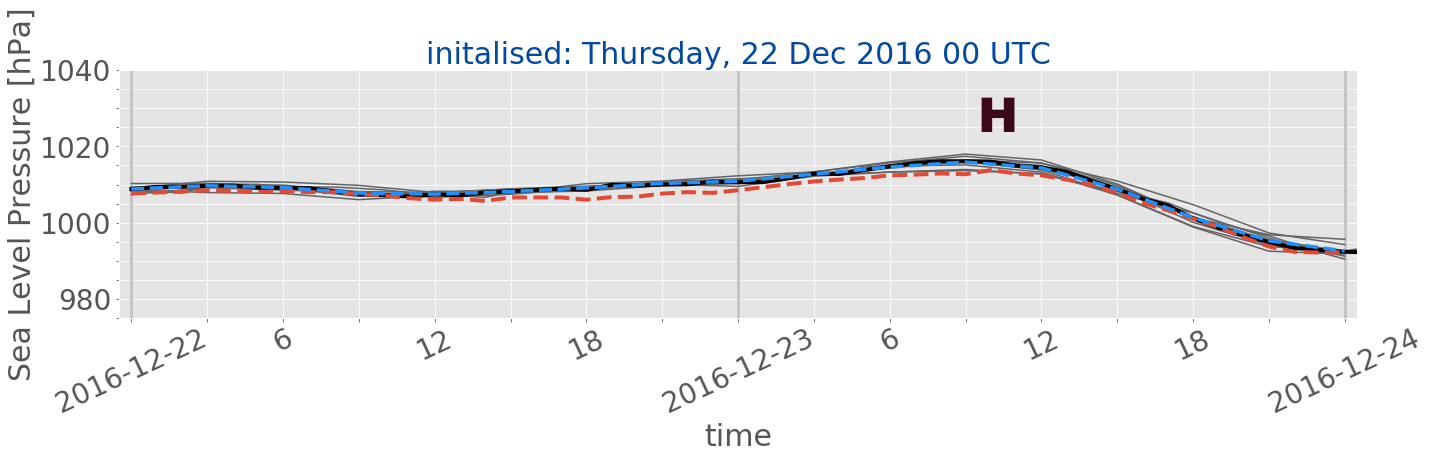
\includegraphics[trim={0.cm 5.cm 0cm 0cm},clip,
		width=\textwidth]{./fig_sfc_pressure/20161222_00}
		\caption{}\label{fig:res:sfc_pres22}
	\end{subfigure}
	% sfc temp
	\begin{subfigure}[b]{0.49\textwidth}
		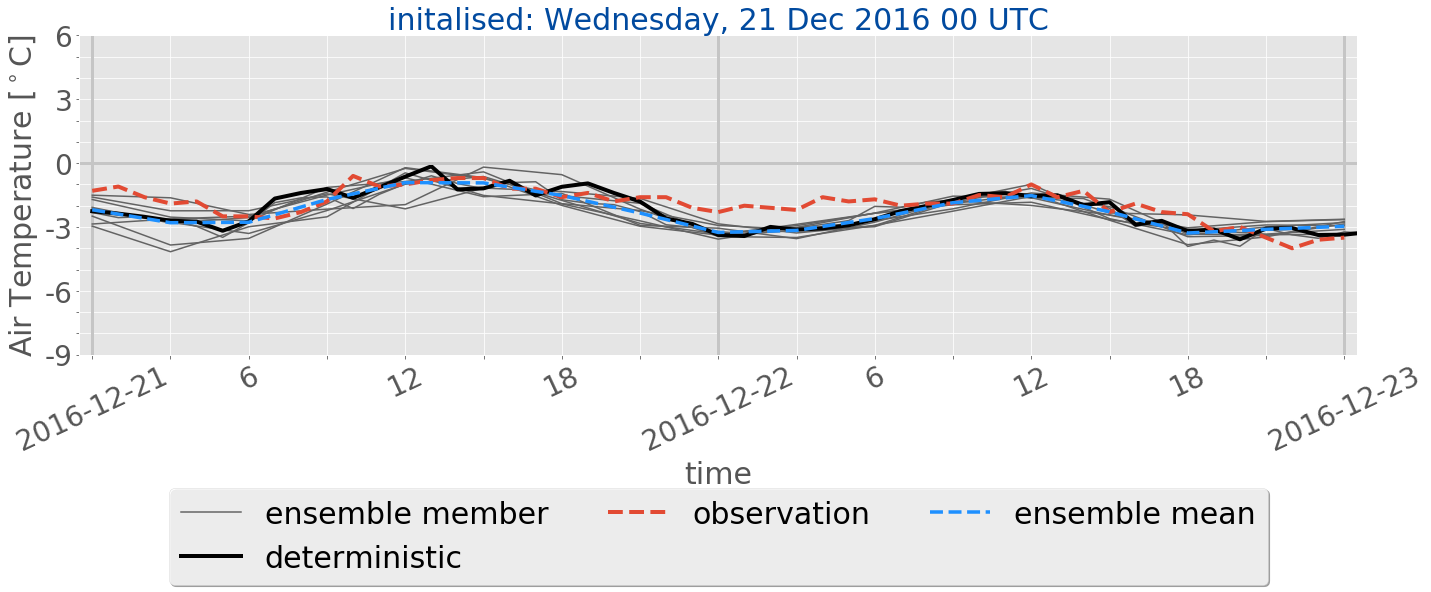
\includegraphics[trim={0.cm 5.cm 0cm 0cm},clip,
		width=\textwidth]{./fig_sfc_temp/20161221_00}
		\caption{}\label{fig:res:sfc_temp21}
	\end{subfigure}
	%
	\begin{subfigure}[b]{0.49\textwidth}
		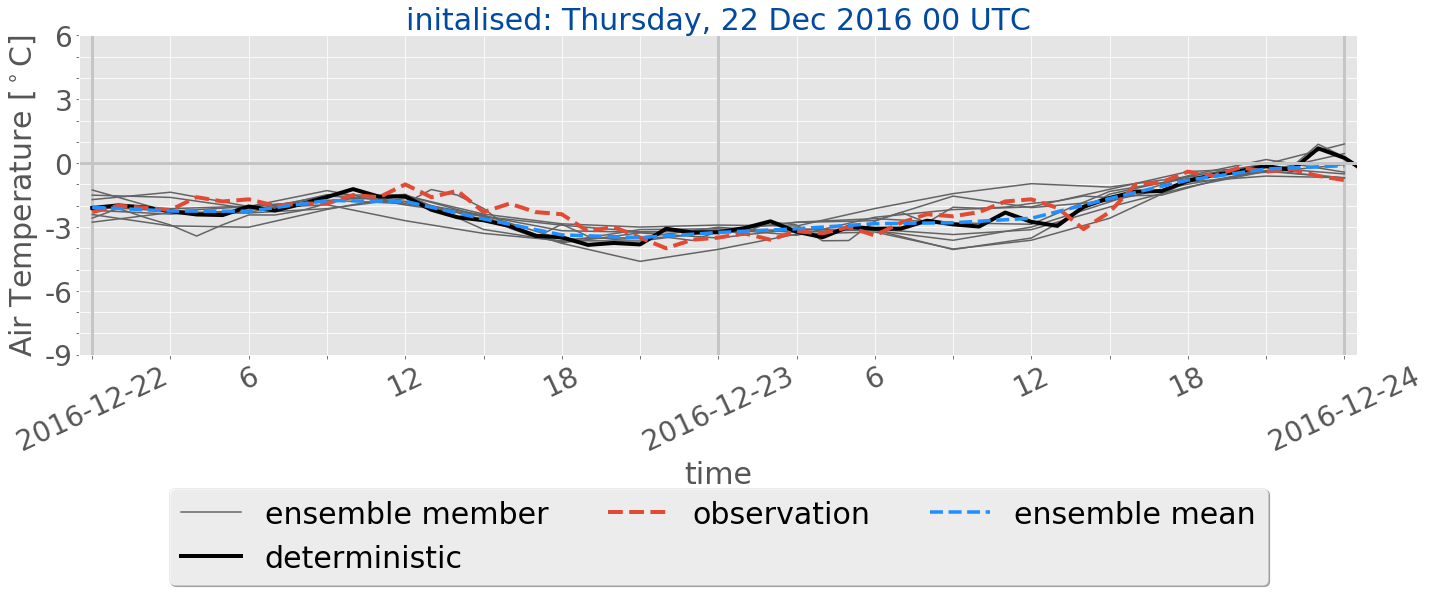
\includegraphics[trim={0.cm 5.cm 0cm 0cm},clip,
		width=\textwidth]{./fig_sfc_temp/20161222_00}
		\caption{}\label{fig:res:sfc_temp22}
	\end{subfigure}
	% sfc wd
	\begin{subfigure}[b]{0.49\textwidth}
		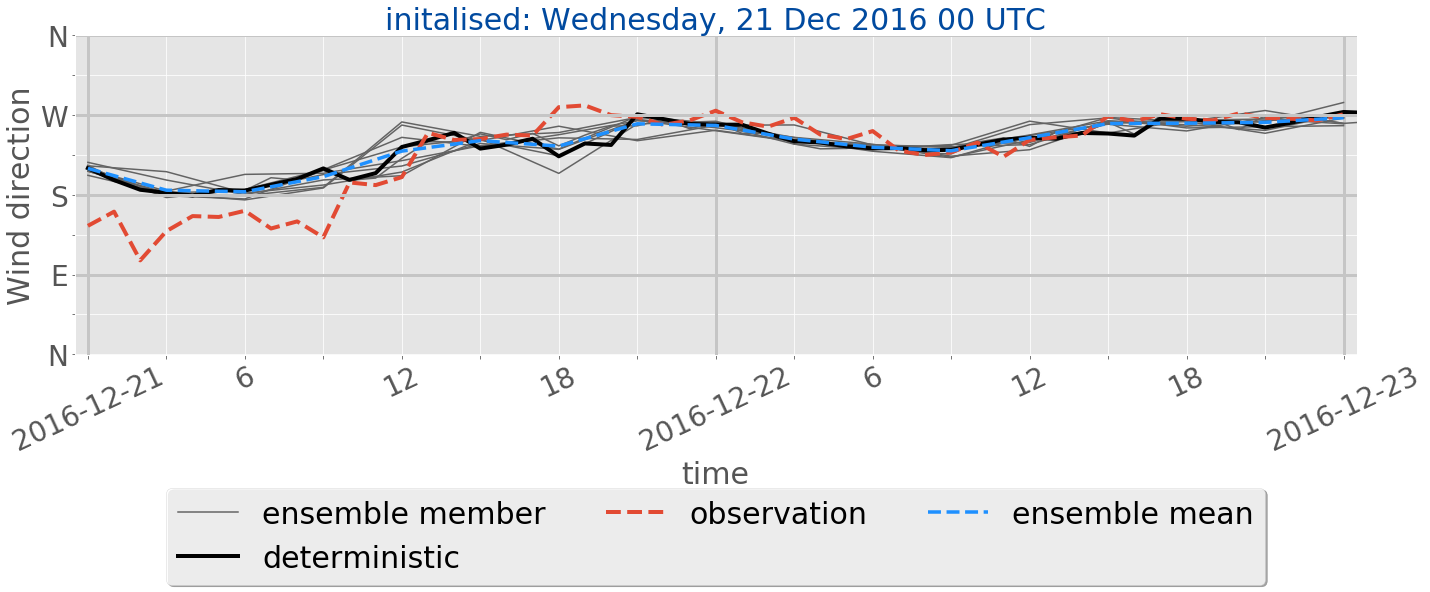
\includegraphics[trim={0.cm 5.cm 0cm 0cm},clip,
		width=\textwidth]{./fig_sfc_wd/20161221_00}
		\caption{}\label{fig:res:sfc_wd21}
	\end{subfigure}
	%
	\begin{subfigure}[b]{0.49\textwidth}
		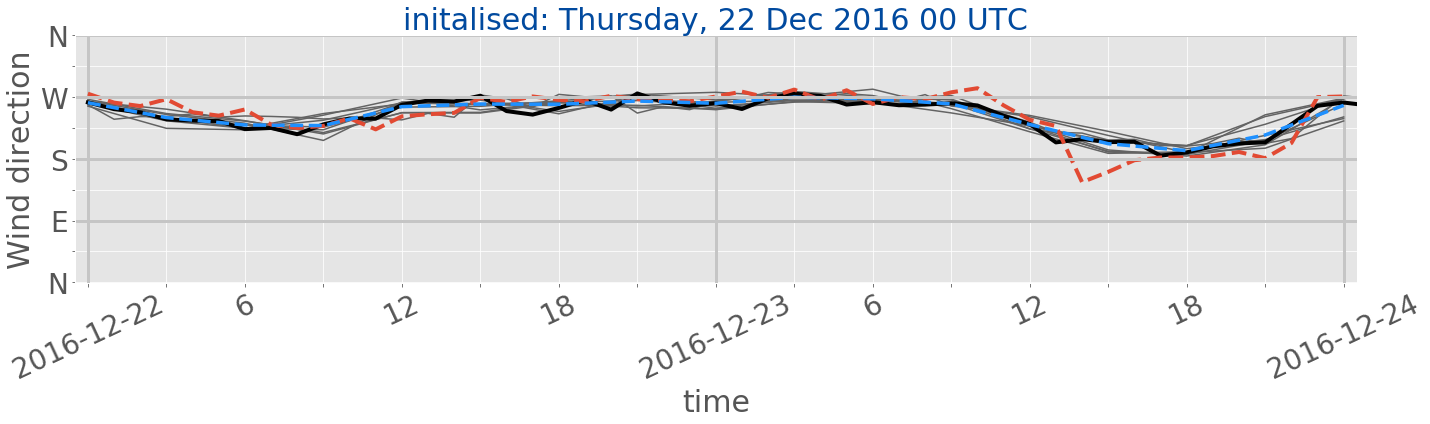
\includegraphics[trim={0.cm 5.cm 0cm 0cm},clip,
		width=\textwidth]{./fig_sfc_wd/20161222_00}
		\caption{}\label{fig:res:sfc_wd22}
	\end{subfigure}
	% sfc ws
	\begin{subfigure}[b]{0.49\textwidth}
		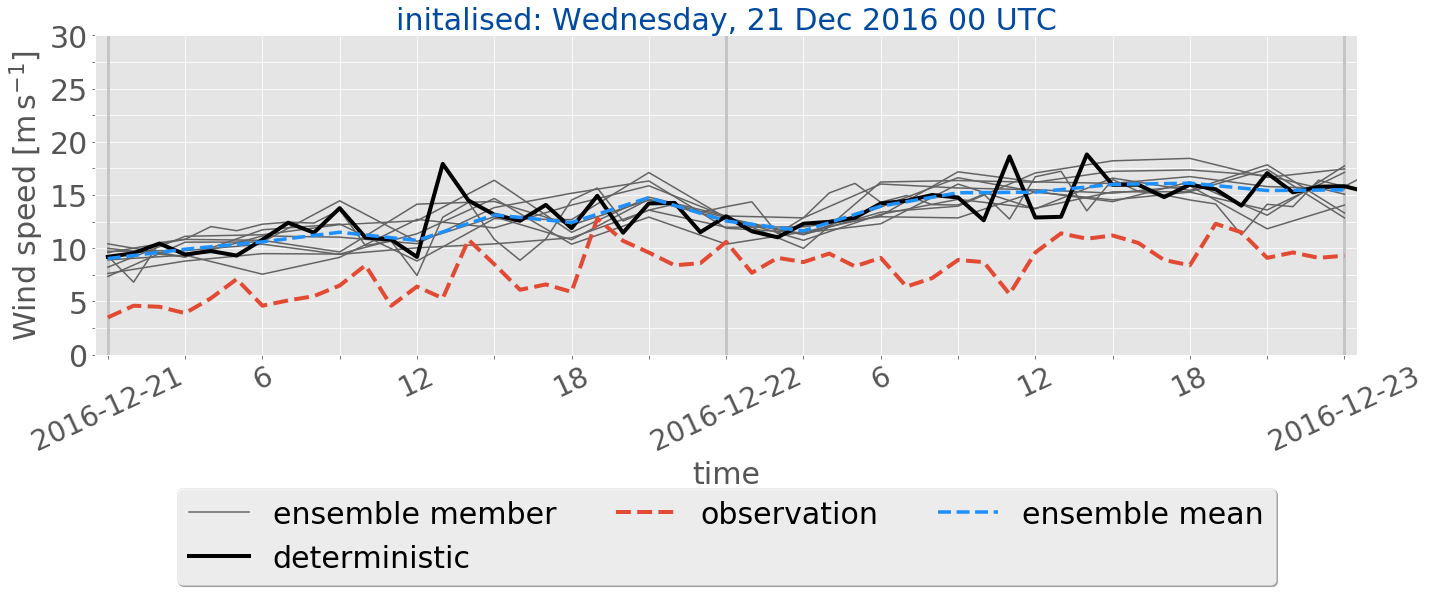
\includegraphics[trim={0.cm 5.cm 0cm 0cm},clip,
		width=\textwidth]{./fig_sfc_ws/20161221_00}
		\caption{}\label{fig:res:sfc_ws21}
	\end{subfigure}
	%
	\begin{subfigure}[b]{0.49\textwidth}
		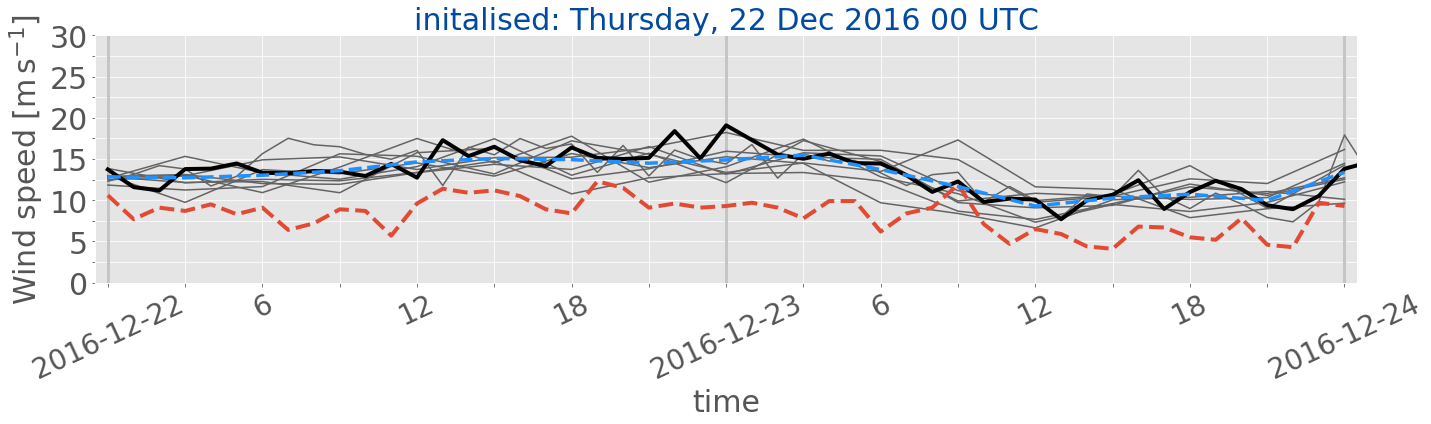
\includegraphics[trim={0.cm 5.cm 0cm 0cm},clip,
		width=\textwidth]{./fig_sfc_ws/20161222_00}
		\caption{}\label{fig:res:sfc_ws22}
	\end{subfigure}
	% sfc precip
	\begin{subfigure}[b]{0.49\textwidth}
		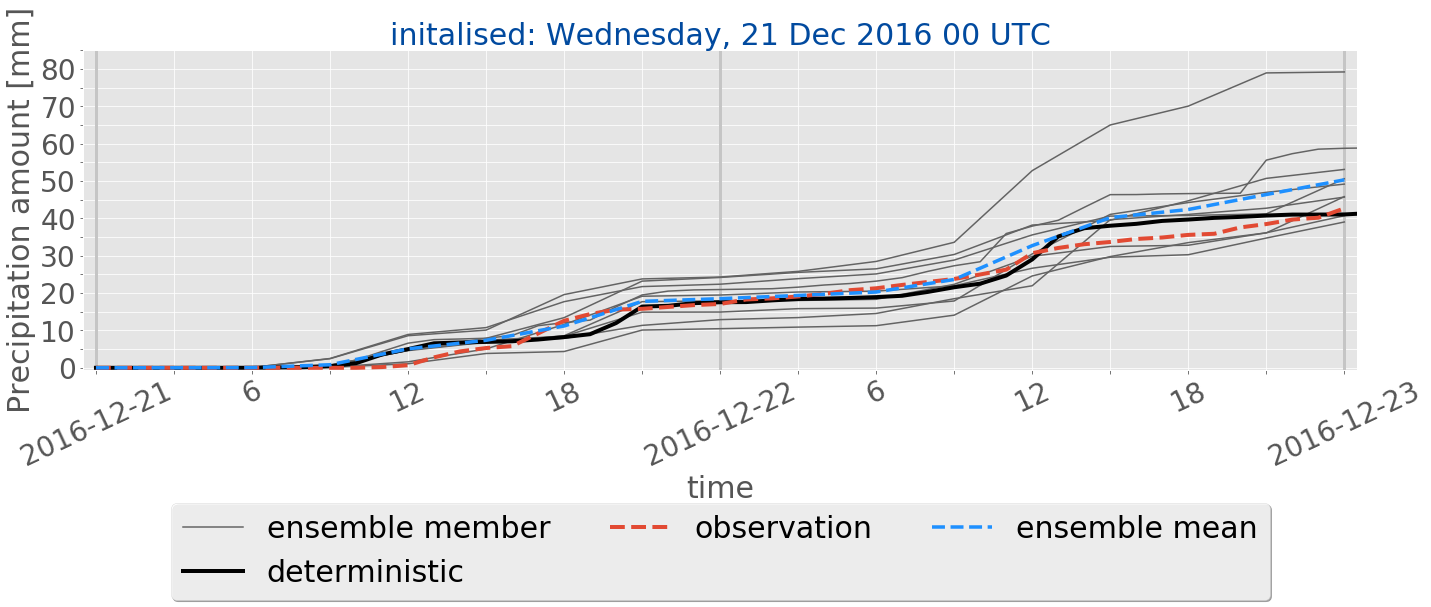
\includegraphics[trim={0.cm 3.6cm 0cm 0cm},clip,
		width=\textwidth]{./fig_sfc_precip/20161221_00}
		\caption{}\label{fig:res:sfc_precip21}
	\end{subfigure}
	%
	\begin{subfigure}[b]{0.49\textwidth}
		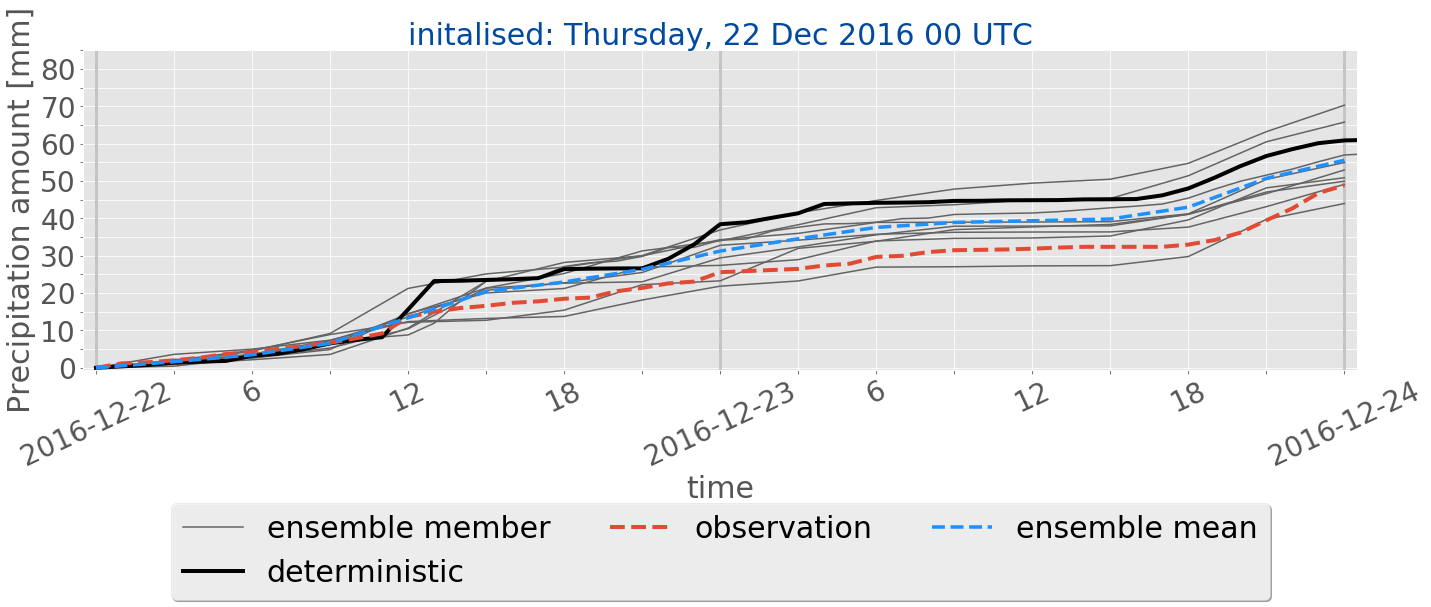
\includegraphics[trim={0.cm 3.6cm 0cm 0cm},clip,
		width=\textwidth]{./fig_sfc_precip/20161222_00}
		\caption{}\label{fig:res:sfc_precip22}
	\end{subfigure}
	
	% label
	\begin{subfigure}[b]{\textwidth}
		\centering
		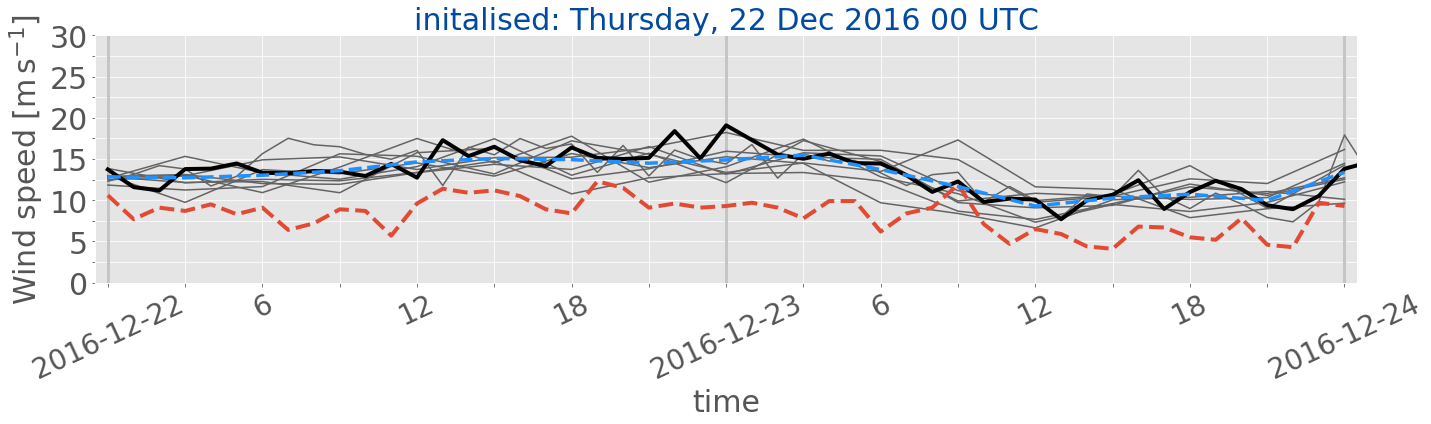
\includegraphics[trim={5.5cm 0cm 5.cm 17.2cm},clip,
		width=0.8\textwidth]{./fig_sfc_ws/20161222_00}
	\end{subfigure}
	%
	\caption{\SI{48}{\hour} surface observations and ensemble forecasts initialised on the \SI{21}{\dec} (left column, \protect\subref{fig:res:sfc_pres21}, \protect\subref{fig:res:sfc_temp21}, \protect\subref{fig:res:sfc_wd21}, \protect\subref{fig:res:sfc_ws21}, \protect\subref{fig:res:sfc_precip21}), and on \SI{22}{\dec} (right column, \protect\subref{fig:res:sfc_pres22}, \protect\subref{fig:res:sfc_temp22}, \protect\subref{fig:res:sfc_wd22}, \protect\subref{fig:res:sfc_ws22}, \protect\subref{fig:res:sfc_precip22}). Line representation according to the label. Upper panel sea level pressure, second \SI{2}{\metre} air temperature, third and fourth \SI{10}{\metre} wind direction and speed, respectively, and lowest panel precipitation amount. }\label{fig:app:sfc_obs_meps}
\end{figure}
\begin{figure}\ContinuedFloat
	\centering
	% sfc pressure
	\begin{subfigure}[b]{0.49\textwidth}
		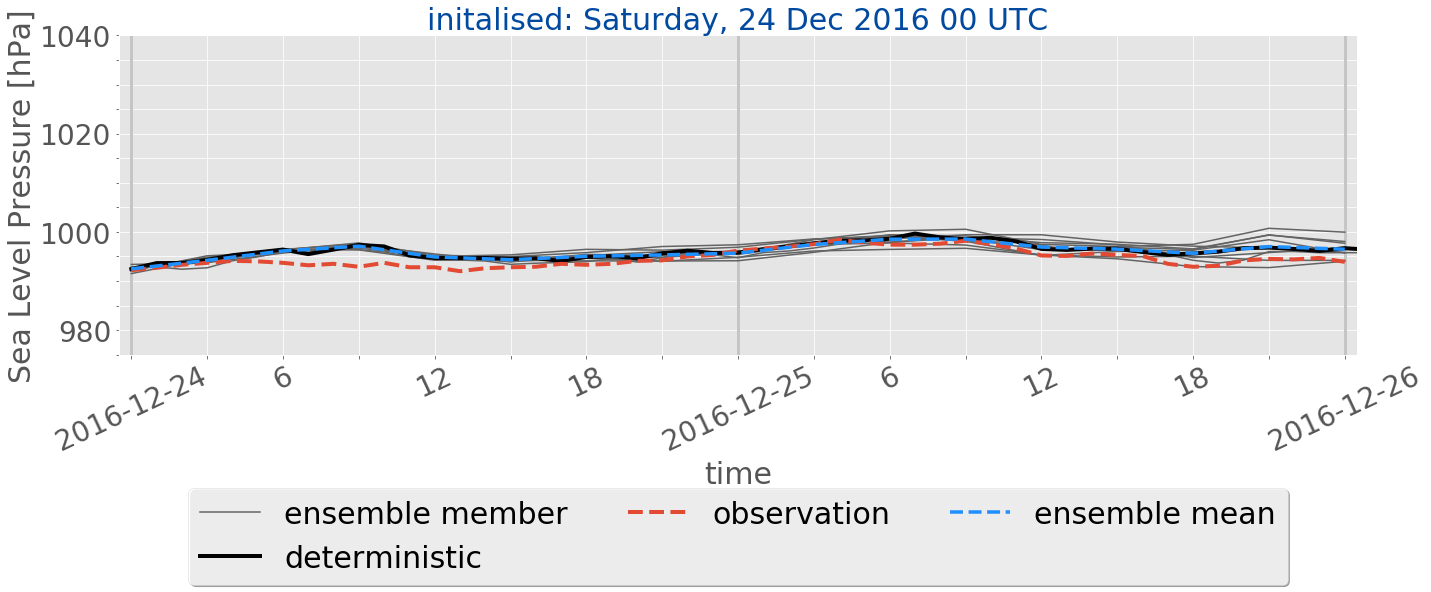
\includegraphics[trim={0.cm 5.cm 0cm 0cm},clip,
		width=\textwidth]{./fig_sfc_pressure/20161224_00}
		\caption{}\label{fig:res:sfc_pres24}
	\end{subfigure}
	
	% sfc temp
	\begin{subfigure}[b]{0.49\textwidth}
		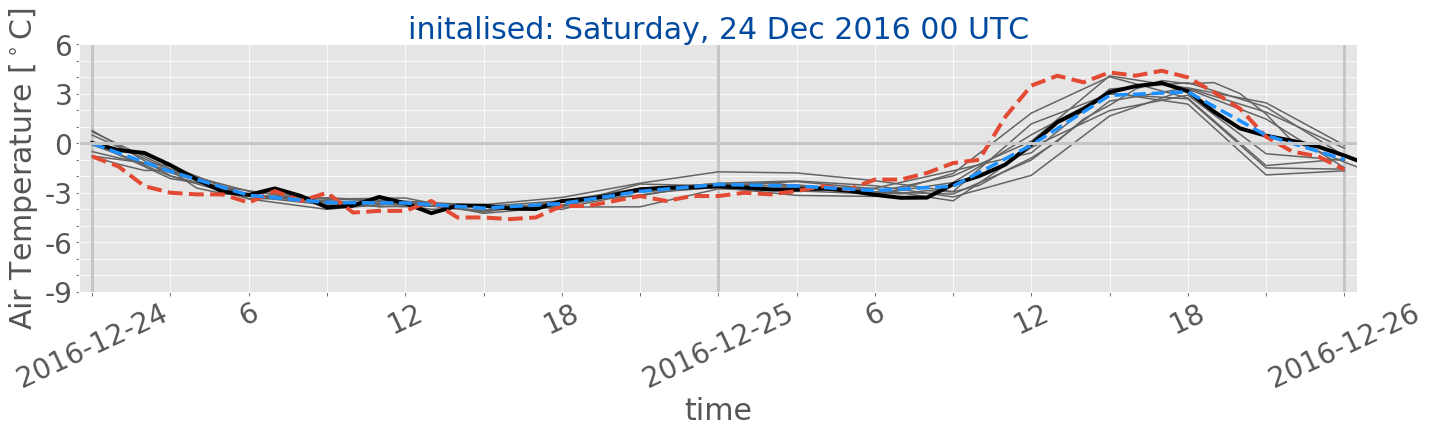
\includegraphics[trim={0.cm 5.cm 0cm 0cm},clip,
		width=\textwidth]{./fig_sfc_temp/20161224_00}
		\caption{}\label{fig:res:sfc_temp24}
	\end{subfigure}
	
	% sfc wd
	\begin{subfigure}[b]{0.49\textwidth}
		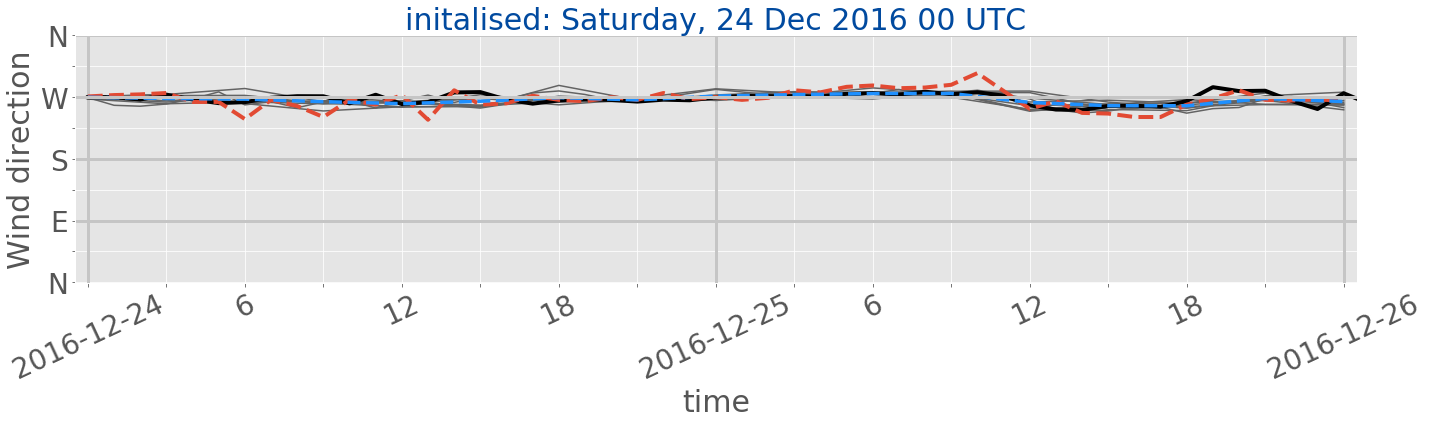
\includegraphics[trim={0.cm 5.cm 0cm 0cm},clip,
		width=\textwidth]{./fig_sfc_wd/20161224_00}
		\caption{}\label{fig:res:sfc_wd24}
	\end{subfigure}
	
	% sfc ws
	\begin{subfigure}[b]{0.49\textwidth}
		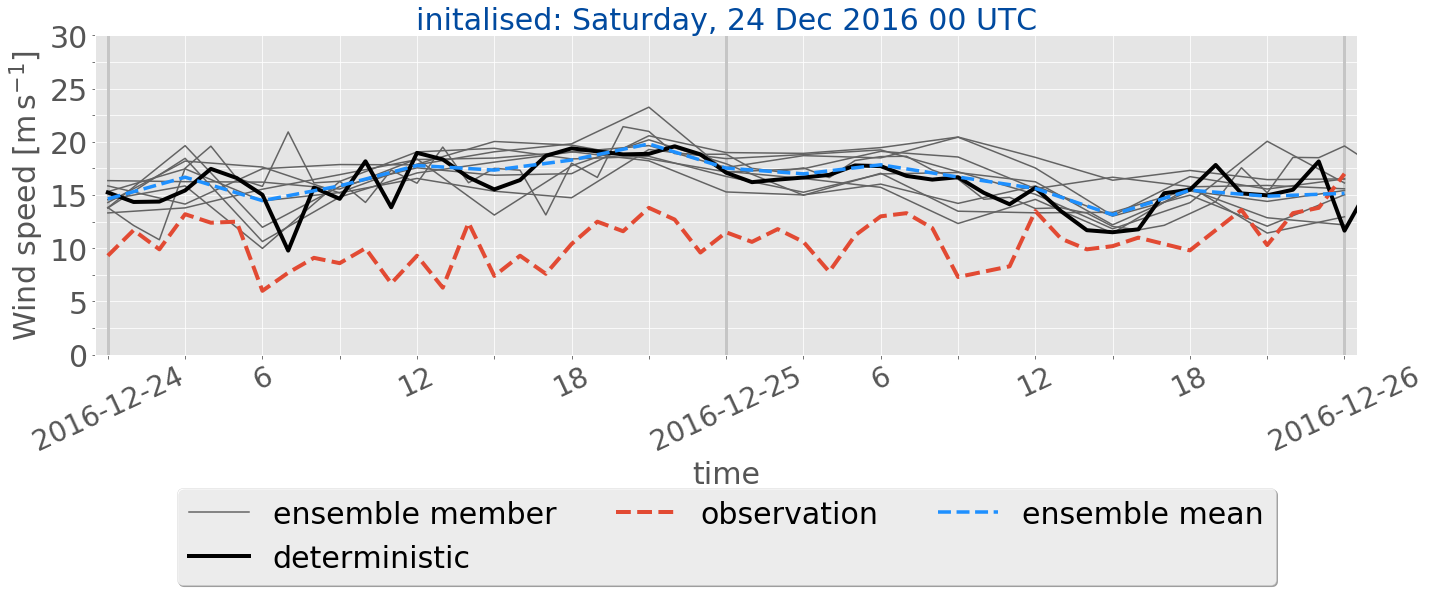
\includegraphics[trim={0.cm 5.cm 0cm 0cm},clip,
		width=\textwidth]{./fig_sfc_ws/20161224_00}
		\caption{}\label{fig:res:sfc_ws24}
	\end{subfigure}
	
	% sfc precip
	\begin{subfigure}[b]{0.49\textwidth}
		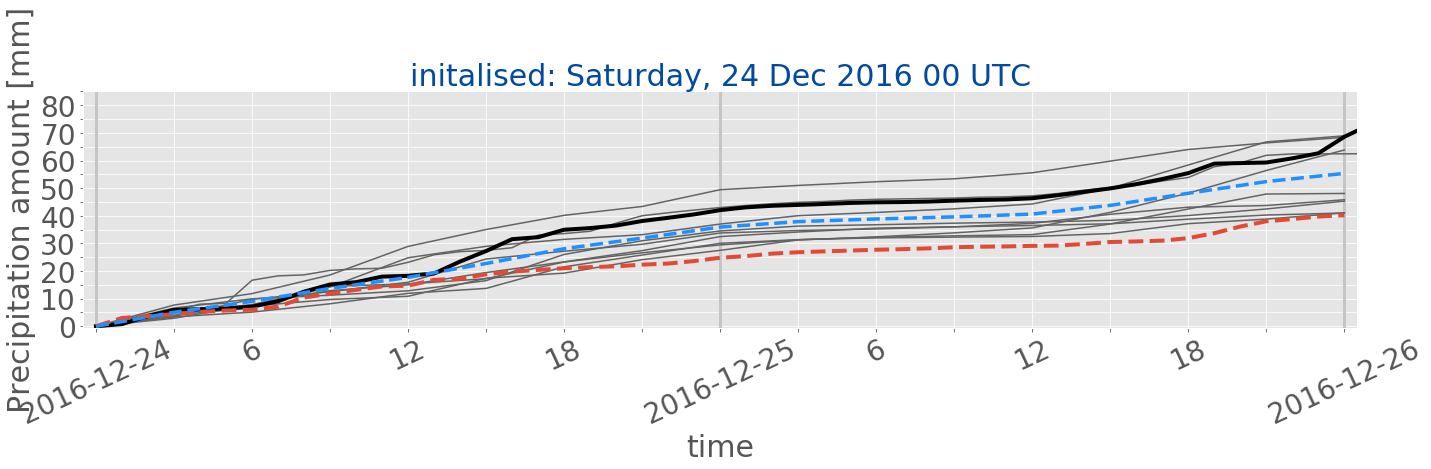
\includegraphics[trim={0.cm 3.6cm 0cm 0cm},clip,
		width=\textwidth]{./fig_sfc_precip/20161224_00}
		\caption{}\label{fig:res:sfc_precip24}
	\end{subfigure}
	
	% label
	\begin{subfigure}[b]{\textwidth}
		\centering
		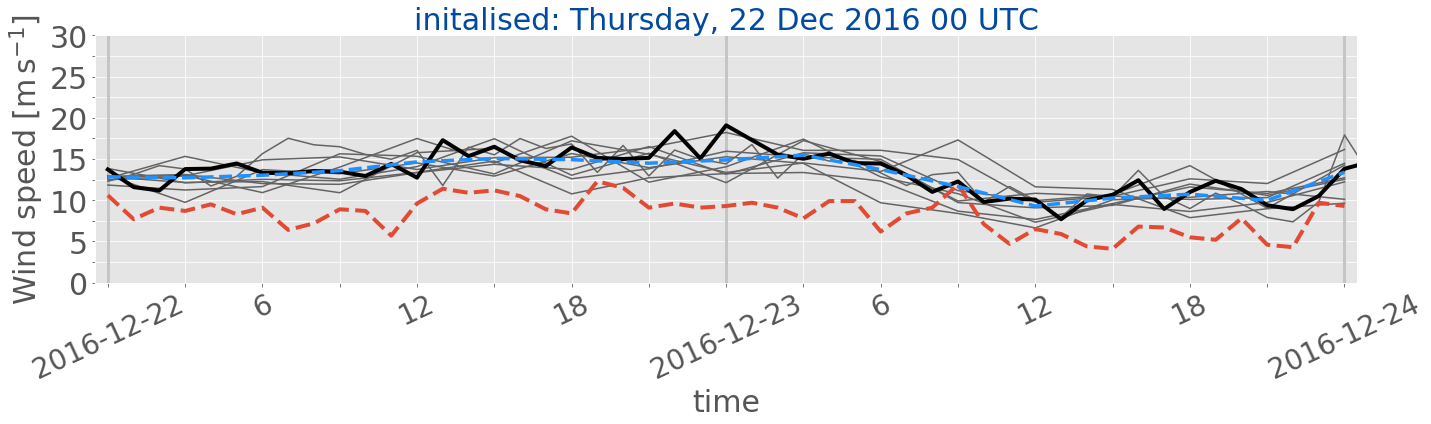
\includegraphics[trim={5.5cm 0cm 5.cm 17.2cm},clip,
		width=0.8\textwidth]{./fig_sfc_ws/20161222_00}
	\end{subfigure}
	\caption{\textit{(Continued from previous page.)} Initialisations for \SI{22}{\dec} (\protect\subref{fig:res:sfc_pres24}, \protect\subref{fig:res:sfc_temp24}, \protect\subref{fig:res:sfc_wd24}, \protect\subref{fig:res:sfc_ws24}, \protect\subref{fig:res:sfc_precip24})}
\end{figure}
%%%%%%%%%%%%%%%%%%%%%%%%%%%%%%%%%%%%%%%%%%%%%%